
\section{Data} \label{Data}

\subsection{Natural Disaster Data}

Natural disasters are declared as such by the president, usually upon request by the affected state's governor. Once a disaster is federally declared, states or local governments can receive federal assistance. The Federal Emergency Management Agency (FEMA) provides data on all federally declared natural disasters, beginning in 1953. The data is easily accessible via their API \citep{rfema}.

Figure \ref{DisasterMap} shows the number of declared disasters between 2009 and 2018 across the US. It seems that the variation in the number of declared disasters may be driven by the governor's proactiveness in requesting a declaration. Thus, it could be interesting to compare counties on different sides of state borders, whose actual disaster exposure is likely very similar in order to analyze the effect of a declaration.


\begin{figure}[!h]
	\centering
	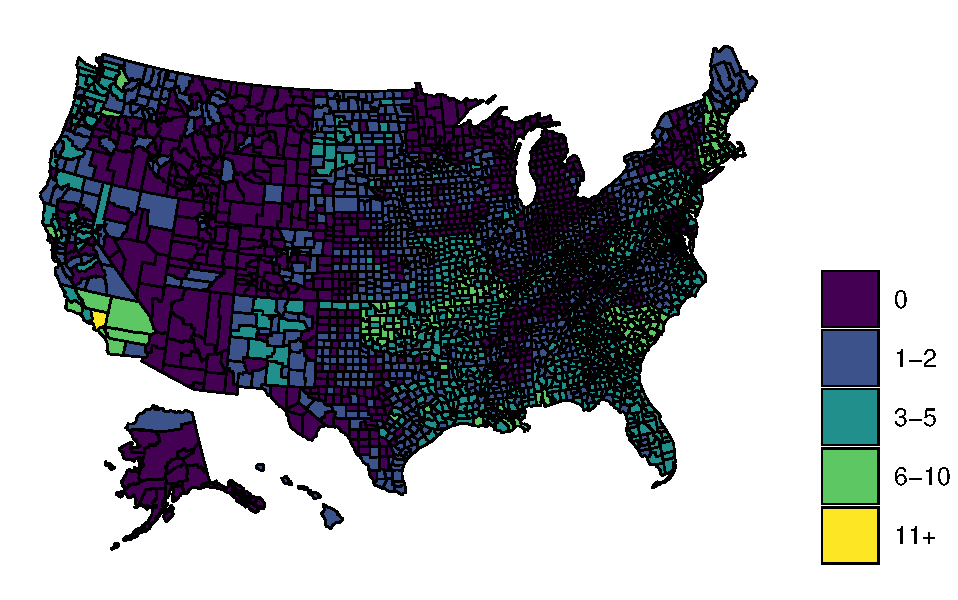
\includegraphics[scale=1]{"../Code & Data/DisasterMap.png"}
	\caption{Number of declared natural disasters from 2009 to 2018}
	\label{DisasterMap}
\end{figure}


FEMA also provides a dataset on  their Public Assistance Applicants Program Deliveries. This contains information on applicants and their recovery priorities, including the amount of damage caused and amount of federal disaster assistance granted. Unfortunately, this data is only available since October 2016. Figure \ref{AssistanceMap} shows the total federal assistance awarded to counties.


\begin{figure}[!h]
	\centering
	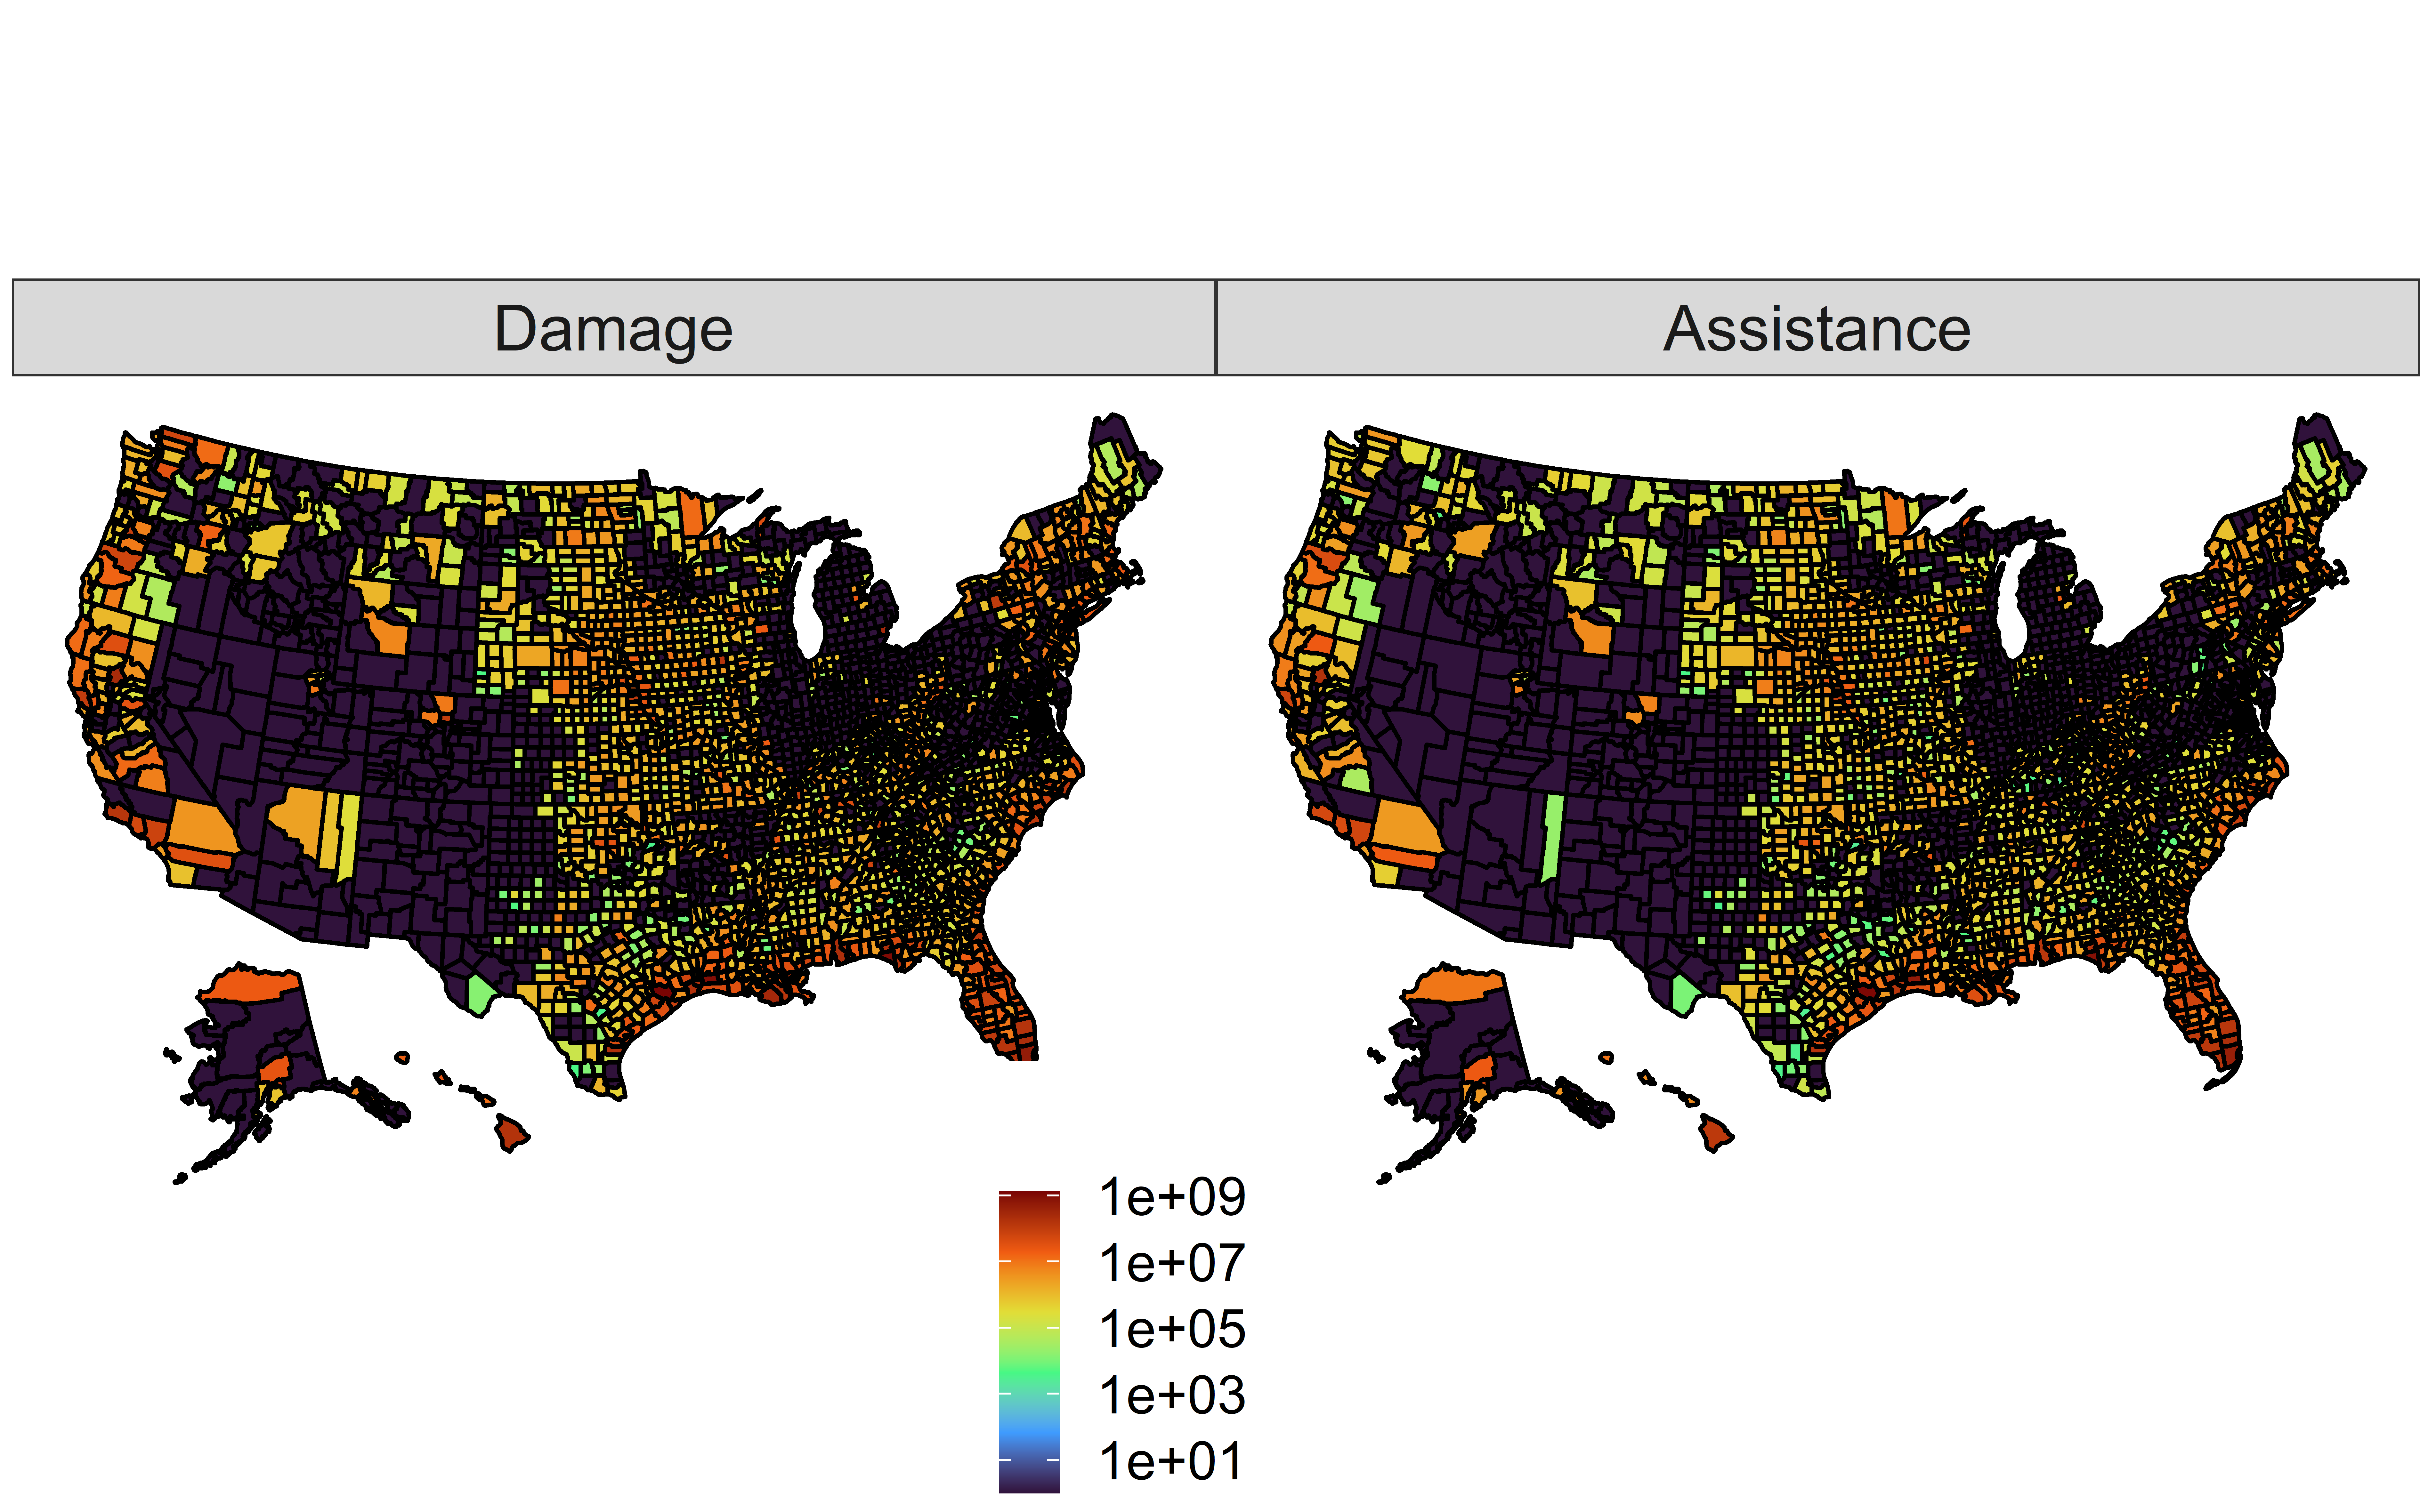
\includegraphics[scale=1]{"../Code & Data/AssistanceMap.png"}
	\caption{Amount of disaster damage and federal disaster assistance (in USD) awarded to counties since October 2016}
	\label{AssistanceMap}
\end{figure}


Figure \ref{AssistCovBoxplot} shows boxplots by county application status. Counties that did apply for federal disaster assistance tend to have lower median income, higher poverty rates, and higher shares of single motherhood. Thus, it seems that counties that had to apply for federal disaster assistance were more socially vulnerable in the first place. However, the direction of causality is not clear. Possibly these counties are more vulnerable to natural disasters and are also poorer or more socially vulnerable because of it. Alternatively, counties that are poorer could be more likely to apply for public disaster aid as they have fewer private resources.

It is also interesting whether variation in the federal assistance procedure may be driven by political factors. Visually, the distribution of democratic votes in the 2016 election (almost coincides with the start of the Public Assistance Applicants Program Deliveries dataset) does not seem to be different in the two groups. However, logistic regression results indicate a significant negative relationship between a county's application status and its share of democratic votes in the 2016 election (see Appendix \ref{AppendixA}). While this is not necessarily a causal effect, it could be an indication that a Republican president may be more hesitant awarding disaster assistance to Democratic counties.

\begin{figure}[!h]
	\centering
	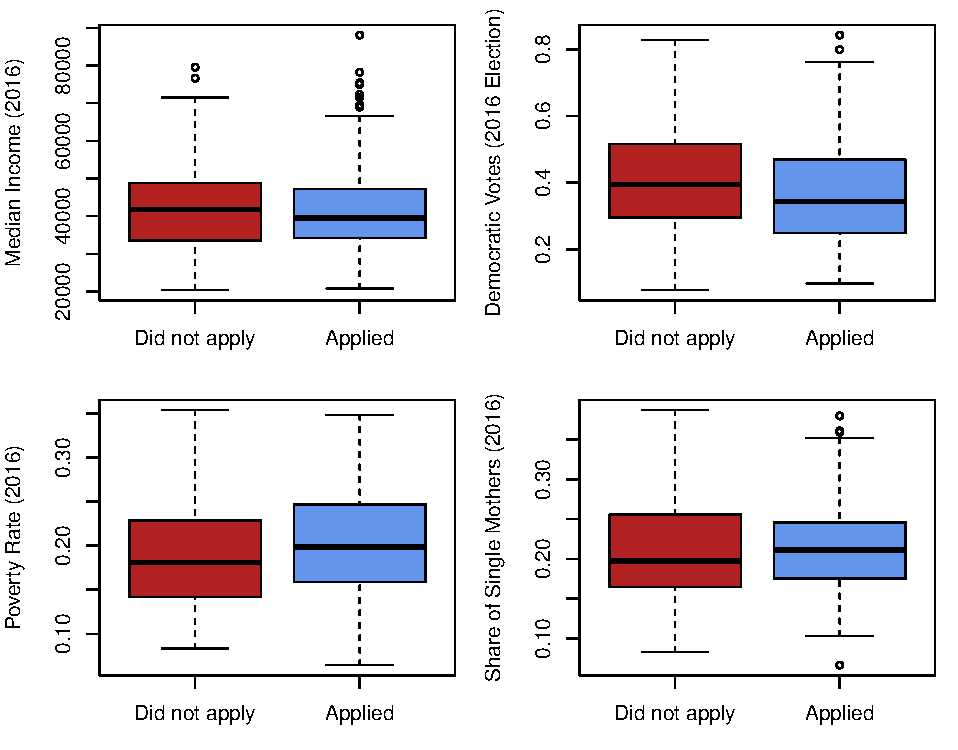
\includegraphics[scale=1]{"../Code & Data/AssistanceCovBoxplot.png"}
	\caption{Boxplots by application status}
	\label{AssistCovBoxplot}
\end{figure}



\subsection{Standardized Testing Data}

Data on academic achievement is available from the Stanford Education Data Archive \citep{SEDA}. They provide mean test results from standardized tests by county, year, grade and subject among all students and various subgroups (including race, gender, and economically disadvantaged). The most recent version 4.1 covers grades 3 through 8 in mathematics and Reading Language Arts (RLA) over the 2008-09 through 2017-18 school years.

Test scores are cohort-standardized, meaning they can be interpreted relatively to an average national reference cohort in the same grade. For instance, a county mean of 0.5 indicates that the average student in the county scored approximately one half of a standard deviation higher than the average national student in the same grade.

In addition to overall mean test scores, the data includes mean test scores for various subgroups, e.g. by ethnicity. In particular, we consider mean test scores for black, hispanic, female, and economically disadvantaged students. These are only reported if the subgroups' sample sizes are large enough. Thus, the number of observations for some of them is substantially smaller.

Furthermore, the Stanford Education Data Archive maintains a large set of covariates for each county and year. They include variables like the county's median income, unemployment and poverty rate.


\subsection{Combining disaster and testing data}

Natural disasters should only have an effect on test scores if they occur before the test. Standardized tests are generally administered during spring. We will use March 1st as a cut-off point. Thus, any disaster happening within the same school year before the 1st of March will be considered. School years tend to start in late August or early September with some variation across states. We will use September 1st, meaning any disaster happening between September 1st and March 1st will be counted for a given school year.

Each disaster is assigned to a school year as described above. Then, disaster and test score data can be merged by school year and county. This yields a panel data set with six grades and two subjects for each county-year combination.

The outcomes of interest are overall mean test scores by county, and mean test scores for black, hispanic, female, and economically disadvantaged students. Table \ref{SumStats} shows summary statistics and figure \ref{DepVarsBoxplot} shows boxplots for the five outcomes of interest. All five mean test scores are measured on the cohort standardized scale, that is a given observation measures the distance in standard deviations from the national reference cohort.

\begin{table}[!htbp] \centering \renewcommand*{\arraystretch}{1.1}\caption{Summary Statistics}\label{SumStats}\resizebox{\textwidth}{!}{
\begin{tabular}{lrrrrrrr}
\hline
\hline
Variable & N & Mean & Std. Dev. & Min & Pctl. 25 & Pctl. 75 & Max \\ 
\hline
Disasters & 331778 & 0.222 & 0.569 & 0 & 0 & 0 & 6 \\ 
Disaster Dummy & 331778 &  &  &  &  &  &  \\ 
... 0 & 278656 & 84\% &  &  &  &  &  \\ 
... 1 & 53122 & 16\% &  &  &  &  &  \\ 
Cumulative Disasters & 331778 & 1.259 & 1.645 & 0 & 0 & 2 & 14 \\ 
Grade & 339264 &  &  &  &  &  &  \\ 
... 3 & 58762 & 17.3\% &  &  &  &  &  \\ 
... 4 & 58660 & 17.3\% &  &  &  &  &  \\ 
... 5 & 57417 & 16.9\% &  &  &  &  &  \\ 
... 6 & 57146 & 16.8\% &  &  &  &  &  \\ 
... 7 & 54538 & 16.1\% &  &  &  &  &  \\ 
... 8 & 52741 & 15.5\% &  &  &  &  &  \\ 
Subject & 339264 &  &  &  &  &  &  \\ 
... Mathematics & 165780 & 48.9\% &  &  &  &  &  \\ 
... RLA & 173484 & 51.1\% &  &  &  &  &  \\ 
Mean test score & 328273 & -0.041 & 0.294 & -3.196 & -0.214 & 0.152 & 1.669 \\ 
White-Black gap & 131047 & 0.618 & 0.256 & -0.754 & 0.454 & 0.771 & 2.358 \\ 
Male-Female gap & 306961 & -0.131 & 0.199 & -1.612 & -0.258 & 0.001 & 1.248 \\ 
Disadvantaged gap & 283272 & 0.543 & 0.211 & -0.995 & 0.413 & 0.669 & 2.052 \\ 
Log Income & 339003 & 10.693 & 0.253 & 9.305 & 10.547 & 10.835 & 11.727 \\ 
Unemployment & 339003 & 0.078 & 0.032 & 0.001 & 0.057 & 0.096 & 0.3\\ 
\hline
\hline
\end{tabular}
}
\end{table}




\begin{figure}[!h]
	\centering
	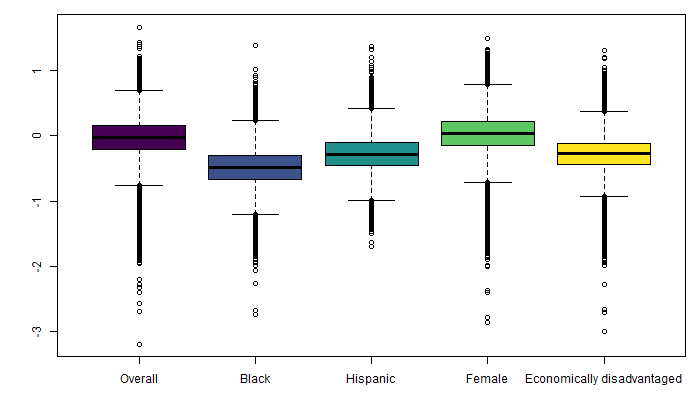
\includegraphics[scale=1]{"../Code & Data/DepVarsBoxplot.png"}
	\caption{Boxplots of the outcomes of interest}
	\label{DepVarsBoxplot}
\end{figure}








